% !TeX program = pdflatex
% !TeX root = NumberOfPolarizations.tex

\documentclass[../FeynCalcManual.tex]{subfiles}
\begin{document}
\hypertarget{numberofpolarizations}{%
\section{NumberOfPolarizations}\label{numberofpolarizations}}

\texttt{NumberOfPolarizations} is an option for
\texttt{DoPolarizationSums}. It specifies the number of polarizations to
sum over in the expression. This is relevant only for expressions that
contain terms free of polarization vectors. This may occur e.g.~if the
scalar products involving polarization vectors have already been
assigned some particular values. In this case the corresponding terms
will be multiplied by the corresponding number of polarizations.

The default value is \texttt{Automatic} which means that the function
will attempt to recognize the correct value automatically by extracting
the dimension \texttt{dim} of the polarization vectors and putting
\texttt{(dim-2)} for massless and \texttt{(dim-1)} for massive vector
bosons. Notice that if the input expression is free of polarization
vectors, the setting \texttt{Automatic} will fail, and the user must
specify the correct dimension by hand.

\subsection{See also}

\hyperlink{toc}{Overview},
\hyperlink{dopolarizationsums}{DoPolarizationSums}.

\subsection{Examples}

\begin{Shaded}
\begin{Highlighting}[]
\NormalTok{PolarizationVector}\OperatorTok{[}\FunctionTok{p}\OperatorTok{,}\NormalTok{ mu}\OperatorTok{]}\NormalTok{ ComplexConjugate}\OperatorTok{[}\NormalTok{PolarizationVector}\OperatorTok{[}\FunctionTok{p}\OperatorTok{,}\NormalTok{ mu}\OperatorTok{]]}
\end{Highlighting}
\end{Shaded}

\begin{dmath*}\breakingcomma
\bar{\varepsilon }^{*\text{mu}}(p) \bar{\varepsilon }^{\text{mu}}(p)
\end{dmath*}

Here the setting Automatic is sufficient.

\begin{Shaded}
\begin{Highlighting}[]
\NormalTok{FCClearScalarProducts}\OperatorTok{[]}\NormalTok{; }
 
\NormalTok{ScalarProduct}\OperatorTok{[}\FunctionTok{p}\OperatorTok{,} \FunctionTok{p}\OperatorTok{]} \ExtensionTok{=} \DecValTok{0}\NormalTok{; }
 
\NormalTok{PolarizationVector}\OperatorTok{[}\FunctionTok{p}\OperatorTok{,}\NormalTok{ mu}\OperatorTok{]}\NormalTok{ ComplexConjugate}\OperatorTok{[}\NormalTok{PolarizationVector}\OperatorTok{[}\FunctionTok{p}\OperatorTok{,}\NormalTok{ mu}\OperatorTok{]]} \SpecialCharTok{+}\NormalTok{ xyz }
 
\NormalTok{DoPolarizationSums}\OperatorTok{[}\SpecialCharTok{\%}\OperatorTok{,} \FunctionTok{p}\OperatorTok{,} \FunctionTok{n}\OperatorTok{]}
\end{Highlighting}
\end{Shaded}

\begin{dmath*}\breakingcomma
\bar{\varepsilon }^{*\text{mu}}(p) \bar{\varepsilon }^{\text{mu}}(p)+\text{xyz}
\end{dmath*}

\begin{dmath*}\breakingcomma
\text{DoPolarizationSums: The input expression contains terms free of polarization vectors. Those will be multiplied with the number of polarizations given by }2.
\end{dmath*}

\begin{dmath*}\breakingcomma
2 \;\text{xyz}-2
\end{dmath*}

Here it is not

\begin{Shaded}
\begin{Highlighting}[]
\NormalTok{DoPolarizationSums}\OperatorTok{[}\NormalTok{xyz}\OperatorTok{,} \FunctionTok{p}\OperatorTok{,} \FunctionTok{n}\OperatorTok{]}
\end{Highlighting}
\end{Shaded}

\begin{figure}[!ht]
\centering
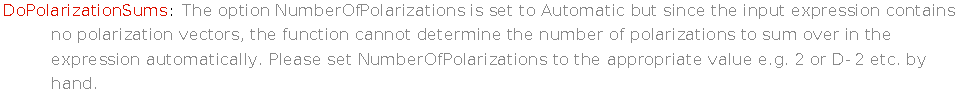
\includegraphics[width=0.6\linewidth]{img/0emyzef54vvcu.pdf}
\end{figure}

\begin{dmath*}\breakingcomma
\text{\$Aborted}
\end{dmath*}

Setting the number of polarizations by hand fixes the issue

\begin{Shaded}
\begin{Highlighting}[]
\NormalTok{DoPolarizationSums}\OperatorTok{[}\NormalTok{xyz}\OperatorTok{,} \FunctionTok{p}\OperatorTok{,} \FunctionTok{n}\OperatorTok{,}\NormalTok{ NumberOfPolarizations }\OtherTok{{-}\textgreater{}} \DecValTok{2}\OperatorTok{]} 
  
 
\end{Highlighting}
\end{Shaded}

\begin{dmath*}\breakingcomma
\text{DoPolarizationSums: The input expression contains terms free of polarization vectors. Those will be multiplied with the number of polarizations given by }2.
\end{dmath*}

\begin{dmath*}\breakingcomma
2 \;\text{xyz}
\end{dmath*}
\end{document}
